\chapter{Implementation}
The landing path generator and the navigation state control system is implememented in the DUNE environment, while controlled and monitored through Neptus. A simplified structure of the autonomous landing system is shown in figure \ref{fig:DuneSystem}. The DUNE task Ardupilot is used as the interface for the Ardupilot in the Pixhawk.
\begin{figure}[H]
	\centering
		\includegraphics[scale=0.8]{figs/DUNESystem.png}
		\caption{A simplified figure of the Dune auto land system}
		\label{fig:DuneSystem}
\end{figure}
\section{Landing plan generator}
The landing plan generator is implemented to be triggered on the consumption of a LandingPlanGeneration \gls{imc} message, which act as the \gls{api} for the task.

The landing path system is implemented in the DUNE task LandingPlan, which is design to start generation of a approach and landing path when receiving the \gls{imc} message LandingPlanGeneration.  The \gls{imc} message was created to structure the parameter needed to construct a flyable approach and landing path. As part of the \gls{imc} message is the ability to specify the rotation direction of the start and finish circle, as well as if there should be a loiter point in the end of the approach path. The ability to specify the rotation direction of the start and final turning circles ensures that the path can be created to take into account environmental obstacles or wind directions. However if all four variants of the approach path is valid, then the shortest path can be chosen by setting the "Automatic" parameter in the LandingPlanGeneration message true. 

The ability to have a loiter manoeuvre at the end of the approach path gives flexibillity when performing a net landing. It allows for final checks of the net condition, or can be used in a dynamic landing operation where the net not stationary e.q. placed on a ship or carried by multi-copters. When configuration the LandingPlan task to perform a dynamical landing only the approach path is created. This was found out to be a preferable solution since a dynamical landing require a feedback loop to correct the desired path, which is currently not included in the landing path system. A solution for performing a dynamical landing is currently research by fellow Master students where the multi-copters is used to catch the \gls{uav}, where this landing system is used to create a approach path to ready the \gls{uav} for a dynamic landing.

The approach path is created as a FollowPath manoeuvre, which is a manoeuvre with a reference position and offset points that displaced relative to the reference position. The distance between each offset point in each arc is given as a task configuration parameter named "Distance Between Arc Segments"
\subsection{Landing plan generation API}
\begin{table}[H]
\centering
\begin{tabular}{| p{2.7cm} | | p{6cm} |}
\hline
\textbf{Parameter name} 							& \textbf{Description} \\ \hline
 Automatic (boolean)								& If true a standard path where the shortest Dubins path is chosen. Otherwise a user specific path is chosen \\ \hline
Start circle turning counter clockwise (boolean)	& If true the start arc is created such that the turning direction is counter clockwise. Otherwise clockwise. Require Automatic==false \\ \hline
Finish circle turning counter clockwise (boolean)	& If true the finish arc is created such that the turning direction is counter clockwise. Otherwise clockwise. Require Automatic==false \\ \hline
Wait at loiter (boolean)							& If true a unlimited loiter is included in the path before the path continue with the path along the virtual runway. \\ \hline

\end{tabular}
\caption{Landing path behaviour setting in LandingPlanGeneration}
\label{Tb:DubinConfig}
\end{table}
\subsubsection{Neptus plug-in}
From Neptus the plug-in LandmapLayer, which is an altered version of Neptus plug-in developed in thesis \citep{Froelich}. Alteration in the plug-in include new parameters, the inclusion of the \gls{imc} message LandingPlangeneration and the ability to manually write the global position coordinates of the net.
\begin{figure}
\centering
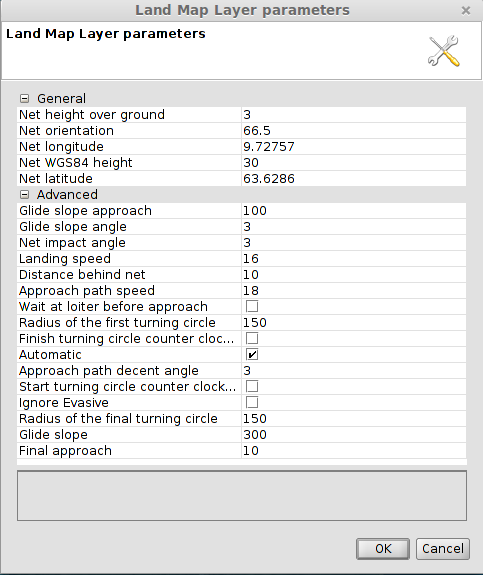
\includegraphics[scale=0.6]{figs/LandMapLayer.png}
\caption{Interaction with the landing plan \gls{api} through Neptus}
\label{Fig:LandMapLayer}
\end{figure}
\subsection{Approach path}
The approach is implemented as a Dubins path from the initial position of the fixed wing \gls{uav} to $\textbf{WP1}$. The approach path creation is started when the landing plan generator receive a LandingPlanGeneration message, which trigger the content extraction of the message. The option for the user to specify the rotation direction of the approach path dictates the system flow 
\begin{figure}[H]
\centering
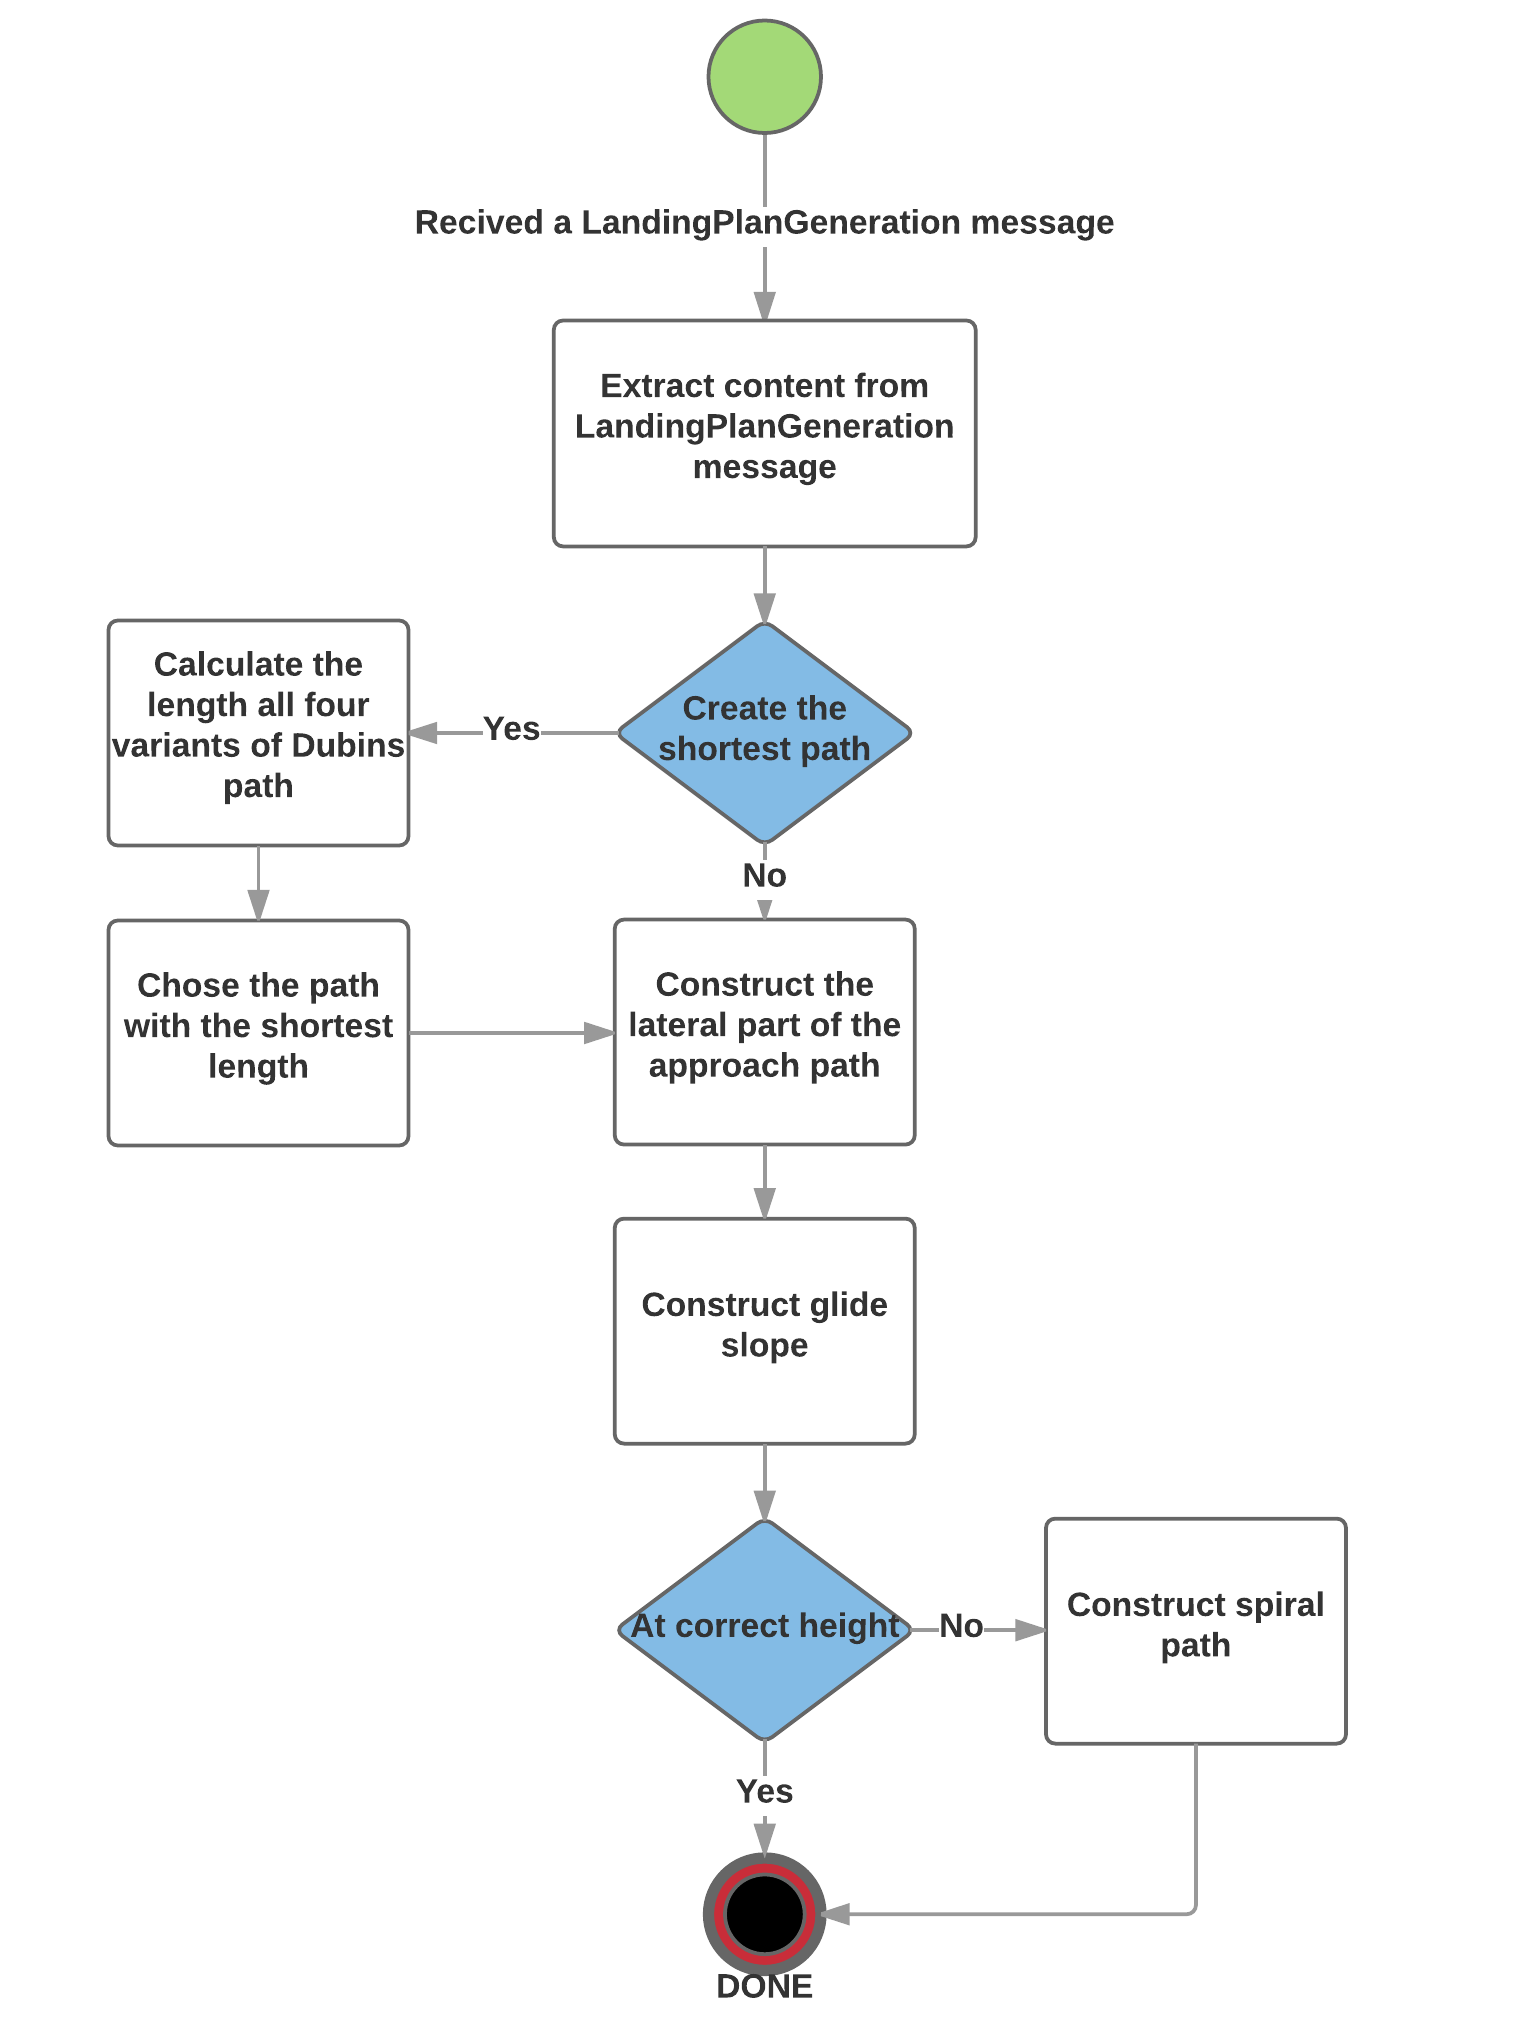
\includegraphics[scale=0.8]{figs/ApproachPath.png}
\caption{Flow chart of approach path creation}
\label{Fig:FlowChartApproach}
\end{figure}
\subsection{Landing path}
The landing path consist of goto manoeuvres, where the position of the goto manoeuvre is given by the way-points $\textbf{WP4-2}$ defined in \ref{SS:netApproach} relative to the position of the net. Figure \ref{Fig:FlowChartLanding} shown the system flow when a landing path is created in the landing plan generator. A option for the landing path is that it includes a loiter manoeuvre at the beginning, which is defined as a circular manoeuvre around a fixed position with a constant radius. The loiter manoeuvre increase the flexibility of the autonomous landing system, by introducing a manoeuvre that in which the \gls{uav} can wait for the landing zone to be prepared. In the case of a dynamic net landing the loiter manoeuvre can be used as a waiting manoeuvre as a final check before the \gls{uav} starts to track the position of the net. An other possible application is to apply the loiter manoeuvre in a net landing where the net is carried by multi-copter \glspl{uav}, where the copters can wait on the ground until the fixed wing \gls{uav} enters the loiter manoeuvre.
\begin{figure}
\centering
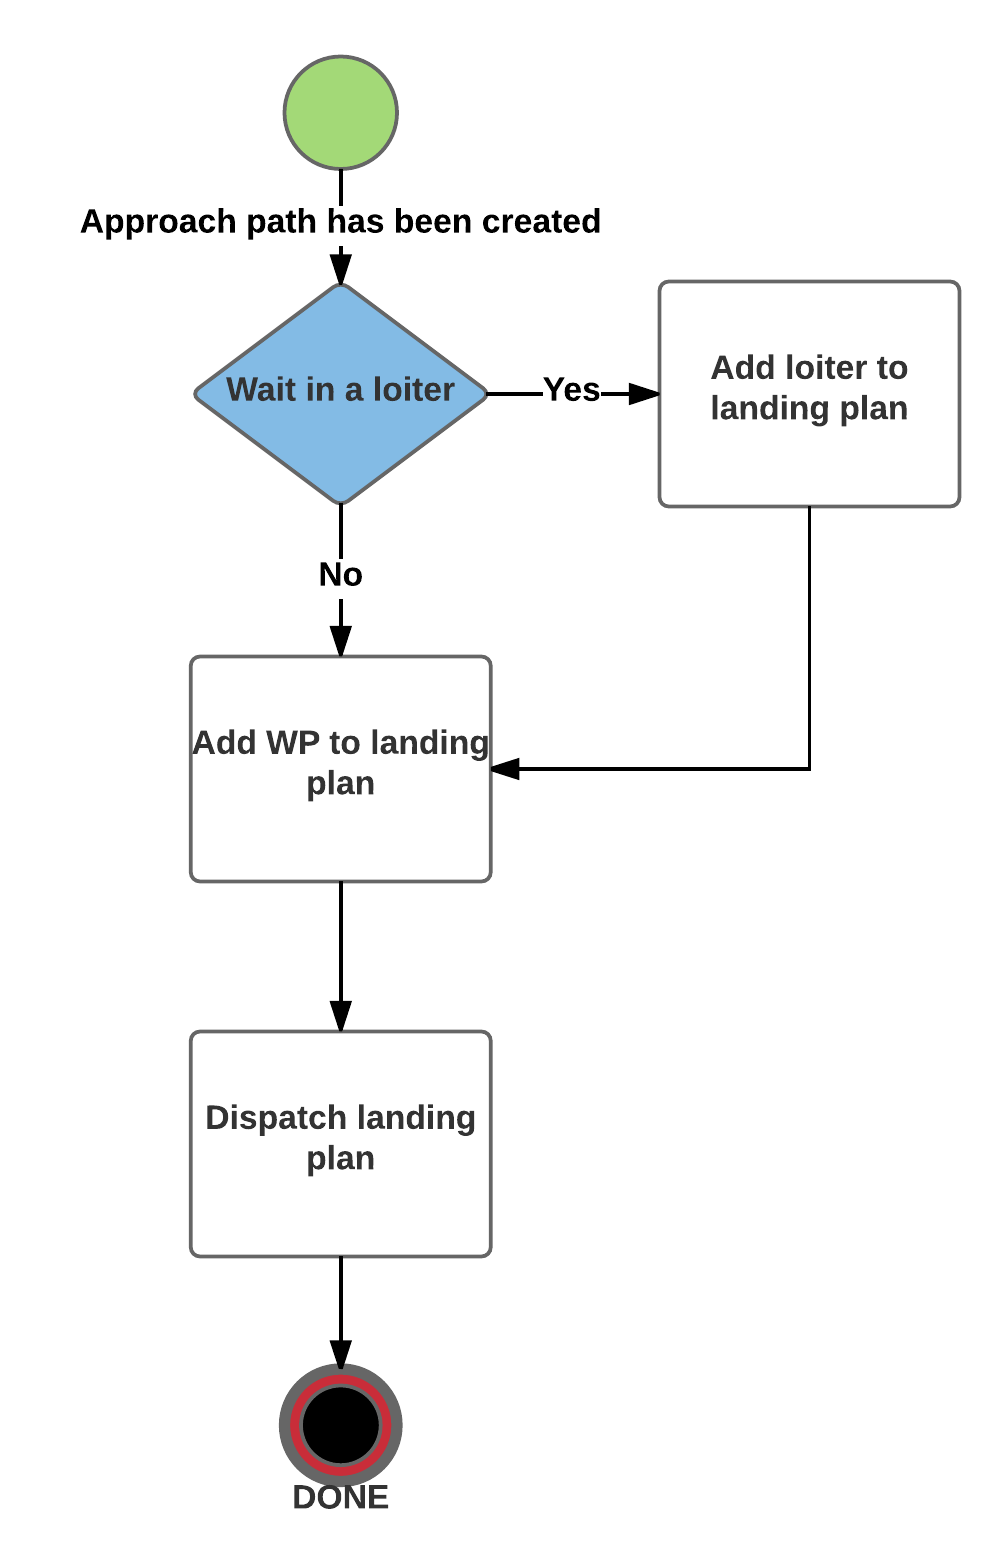
\includegraphics[scale=0.8]{figs/LandingPath.png}
\caption{Flow chart of the landing plan generation}
\label{Fig:FlowChartLanding}
\end{figure}
\subsection{Software in the loop simulation}
The landing plan was tested in a Software In the Loop (SIL) simulation, where the landing plan generation code runs as if it's connected to the actual hardware. The SIL simulation is used to verify that the code function as it's design to do. During a SIL simulation Ardupilot enters a simulation mode, where the JSBSim simulation is used as replacement of the actual X8 fixed wing \gls{uav}. The result obtain from the simulation can be used as a ideal test can of which the performance during a real flight can be compeered against. However the current model of X8 used in the simulation has not been completely verified, such that model error is expected.

A landing path was created to simulate a real landing, where the lateral path is shown in figure \ref{Fig:SILNorthEast090145} and the height versus the desired height is shown in figure \ref{Fig:SILHeight6juni090145}. The plan is designed to fit a operational area where the \gls{uav} will be within the line of sight of the pilot at any time during execution of the landing plan.
\begin{figure}[H]
\centering
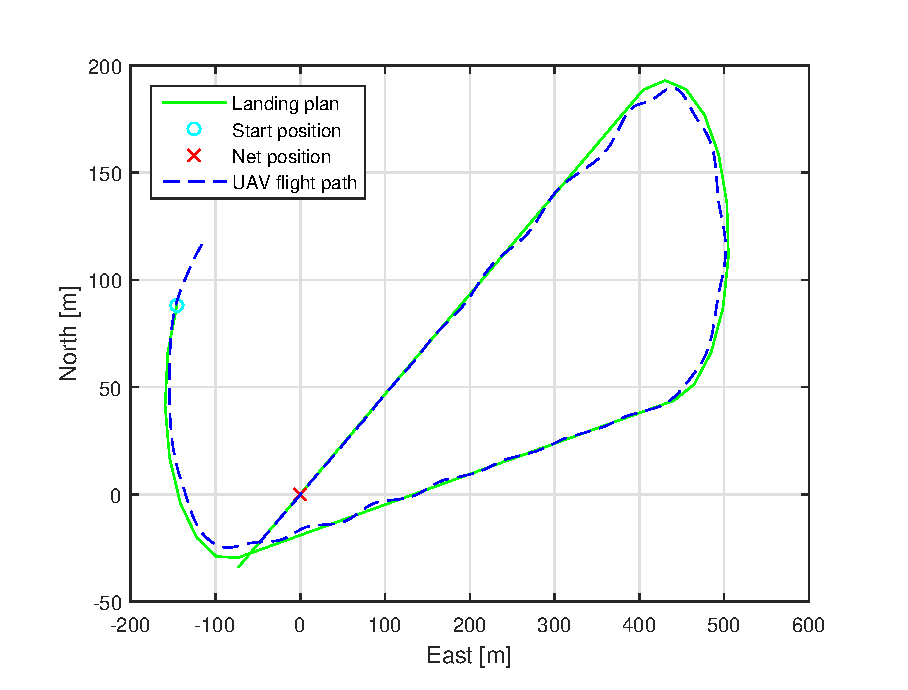
\includegraphics[scale=0.7]{figs/SysPlot/SILNorthEast6juni090145.eps}
\caption{North-East plot of a SIL simulation of the autonomous landing system.}
\label{Fig:SILNorthEast090145}
\end{figure}
\begin{figure}[H]
\centering
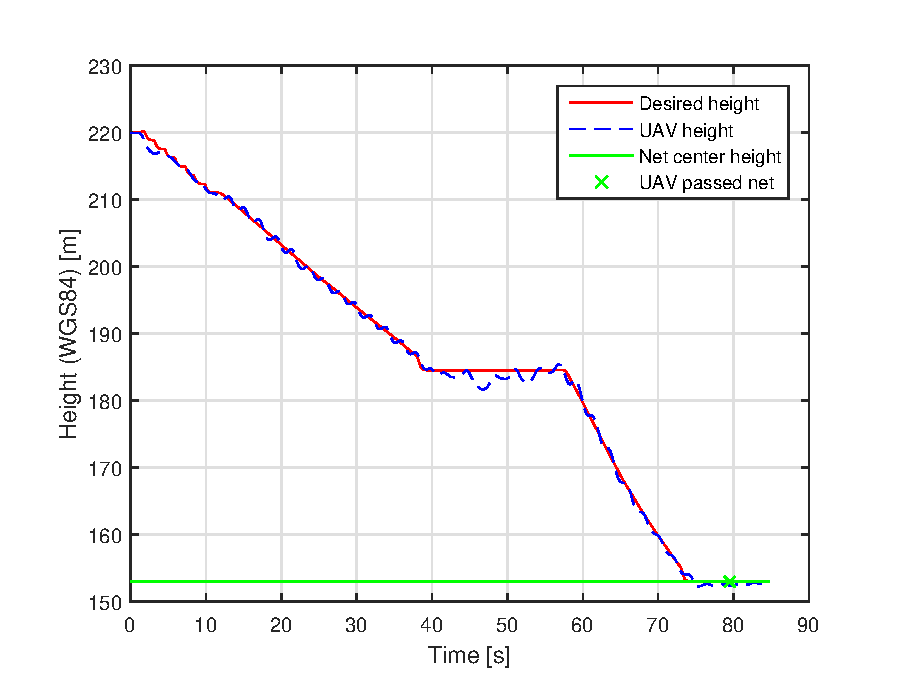
\includegraphics[scale=0.7]{figs/SysPlot/SILHeight6juni090145.eps}
\caption{The desired height and \gls{uav} height when executing the landing plan.}
\label{Fig:SILHeight6juni090145}
\end{figure}
In the case where at the end of the approach path the height does not match the start height of the landing path a downwards spiral is created in order to reach the correct height.

In figure \ref{Fig:SILNorthEastSpiral092307} the spiral function of the lateral path was tested, with the resulting height profile in figure \ref{Fig:SILHeightSpiral092307}. The simulation was performed with a wind disturbance of $9 m/s$ from west, in order to observe how the \gls{uav} would behave during a simulated landing plan with wind disturbance. The lateral guidance system struggles when flying with the wind, however when flying against the wind it's able to stay on the straight line between the way-points. During the turn in the spiral the lateral guidance system is unable to stay on the circle, thus overshooting the desired path. The longitudinal guidance and control system behave similar to the simulation without wind. This indicate that during a actual flight the wind will affect the error in the longitudinal guidance and control system less then the lateral control and guidance system. 
\begin{figure}[H]
\centering
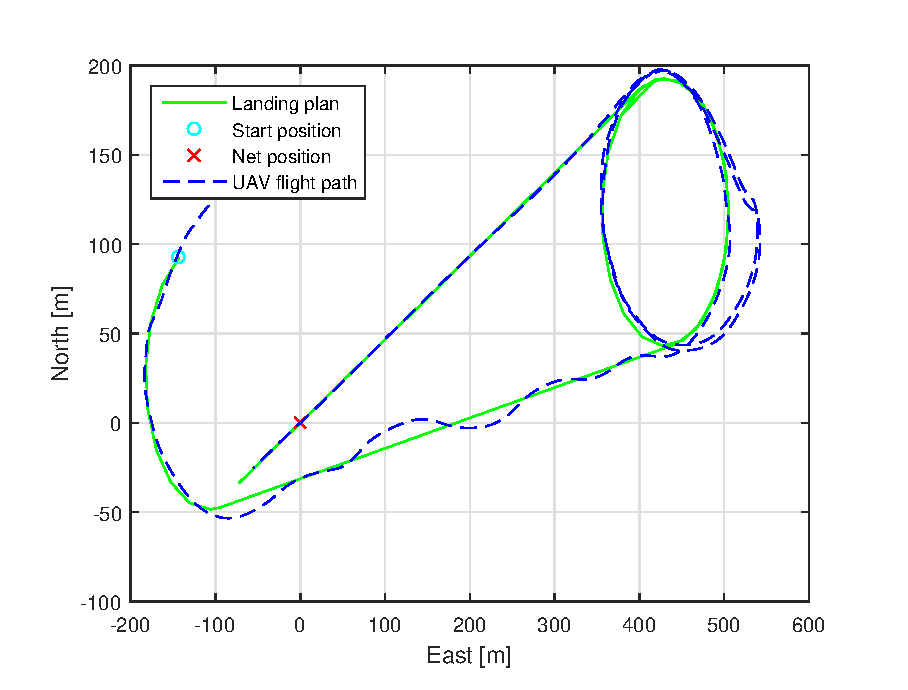
\includegraphics[scale=0.7]{figs/SysPlot/SILNorthEast6juni092307.eps}
\caption{North-East plot where the approach path enters a spiral in order to find a path to the correct height. The simulation was performed with $9 m/s$ wind from west}
\label{Fig:SILNorthEastSpiral092307}
\end{figure}
\begin{figure}[H]
\centering
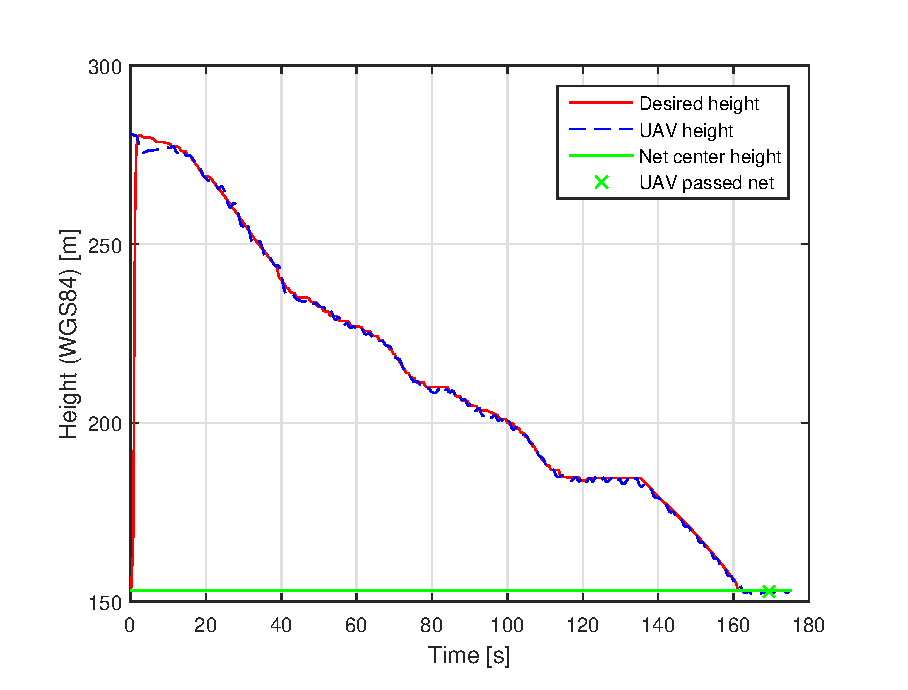
\includegraphics[scale=0.7]{figs/SysPlot/SILHeightSpiral6juni092307.eps}
\caption{The desired height and \gls{uav} height when executing the landing plan from a height that trigger a spiral path towards the correct height with maximum decent angle $\gamma_{d_{Max}}$. The simulation was performed with $9 m/s$ wind from west}
\label{Fig:SILHeightSpiral092307}
\end{figure}
\subsubsection{Result of simulations}
\begin{figure}[H]
\centering
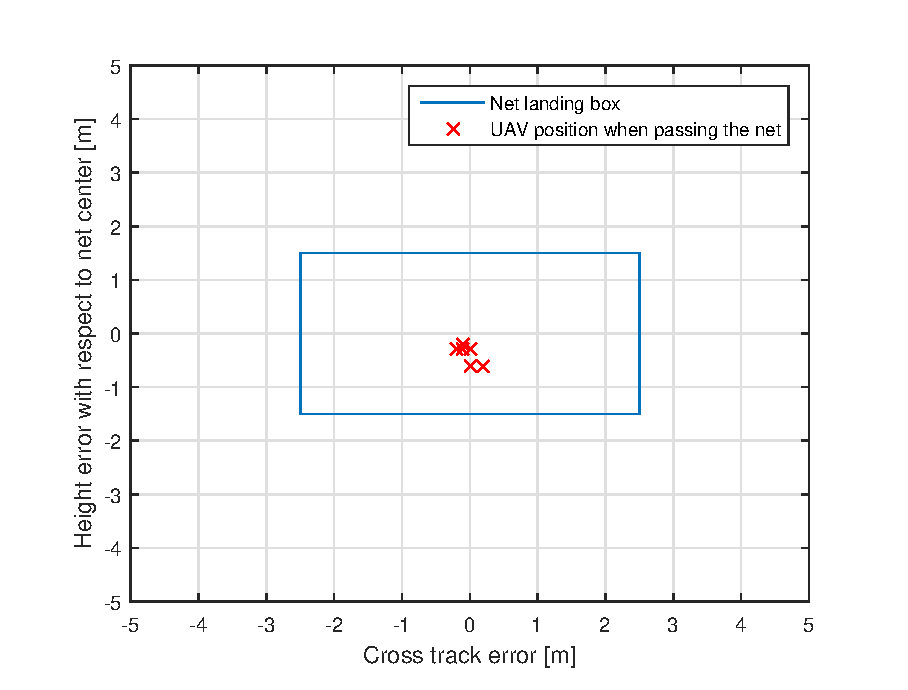
\includegraphics[scale=0.7]{figs/SysPlot/SILNetPasing.eps}
\caption{\gls{uav} position at time of net passing during SIL simulation.}
\end{figure}
\begin{table}[H]
\centering
\begin{tabular}{| l | l | l |}
\hline
\textbf{Nr.} 	& \textbf{Average height error [m]} 	& \textbf{Average cross track error [m]}  \\ \hline
$1$				& $-0.3$							& $-3.1$								\\ \hline
$2$				& $0.7$							& $-4.0$								\\ \hline
$3$				& $0.2$							& $-3.3$								\\ \hline
$4$				& $0.5$							& $-1.2$								\\ \hline
$5$				& $0.4$							& $-2.5$								\\ \hline
$6$				& $0.2$							& $0.3$								\\ \hline
\end{tabular}
\end{table}

\section{Navigation system}
The navigation system is control by a state machine \ref{S:NavState}, which is used to control the content of the output \gls{imc} messages EstimatedState and NavSources. Depending on which state the navigation system is in the \gls{imc} EstimatedState message will either have position solution form the \gls{rtk-gps} system or the external navigation system. During a short loss of the RTK the external navigation position is compensated with the average difference between the RTK solution and the external navigation solution.
\subsection{RTK-GPS system}\label{ss:RTK-GPS system}
The \gls{rtk-gps} solution is dispatched from the DUNE task RTKGPS, however before the message is accepted by the Navigation task the message must include a valid base station position. The base station position is not included in the output message from RTKlib, which demand the base station position to be calculated locally at the base station as a standalone \gls{gnss} receiver. For this purpose the DUNE task BasestationFix is used to lock the current position of the base station, which result in the base station position being transmitted to the RTKGPS task.
The navigation system require to now the reference position of the base station in order to use the \gls{rtk-gps} solution. However the base station position is currently not part of the output message from rtkrcv. This is resolved by allowing the base station to calculate it's own position as a standalone \gls{gps}. The \gls{gps} position is transmitted to a local Dune task on the base station, where the operator can decide when the base station can be considered as fixed. When the base station is considered fixed the position is sent to the X8, where it's included in the \gls{rtk-gps} solution message.
\subsection{State machine}
\subsubsection{Nest system}
A nest system is a stationary unit with the sole purpose of providing it's position to the rest of the Dune System. As part of the navigation system the base station is defined as a nest, where the \gls{gps} position is sent to the \gls{rtk-gps} system when fixed.
An other nest has been created to obtain the \gls{gps} position of the stationary net. The net nest is configured as a rover in \gls{rtk-gps} configuration, such that the position relative to the base station is in the same frame as the X8.
\subsection{Operator interface}
The state of the navigation system is monitored though a interface in Neptus. The interface indicate which source the Dune system is using for state information. The interfaced apply a color code to indicate which source is currently in use in addition to all sensor system that are available, as seen in table \ref{Tb:Color Code}.
\begin{table}[H]
\begin{center}
    \begin{tabular}{ | l | l |}
    \hline
    \textbf{Color} & \textbf{Description} \\ \hline
    White & Not available \\ \hline
    Yellow & Available, but not in use \\ \hline
    Green & Available, and in use \\ \hline
    \end{tabular}
\end{center}
\caption{Net approach parameters }
\label{Tb:Color Code}
\end{table}
\begin{figure}
\centering
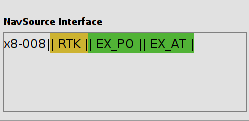
\includegraphics[scale=0.6]{figs/NavSourceInterface.png}
\caption{Navigation source interface}
\label{Fig:NavsourceInterface}
\end{figure}
\section{Summary}